Recently seawater intrusion has become a significant problem in coastal regions.  As populations
increase in these regions, natural recharge no longer counteracts the effects of withdrawals, and so
it is important to have a tool that can estimate the amount of seawater intrusion that may occur
with the continued withdrawal from coastal aquifers. Several numerical models have been developed to
address seawater intrusion in coastal aquifers, and so it is important to have an analytic solution
to use as a benchmark. The benchmarking of numerical code against analytic solutions is a necessary
step in verifying the correctness of the numerical approximations \cite{Simpson}.

Henry's Problem has been widely used as a benchmark case for seawater intrusion numerical models. A
number of numerical solutions have given nearly identical results for Henry's Problem; however no
numerical model to date has been able to match the Henry Solution \cite{Voss}. Henry's Semi-Analytic
Solution to Seawater Intrusion has been tempered by both the inability to use, powerful computing
technologies, which has become readily available to researchers, and a lack of a sufficient number
of Fourier coefficients, so as to ensure a smooth convergence.  In fact, S\'egol \cite{Segol}
suggested that discrepancies between Henry and her own solutions may have been a result of a lack of
convergence in Henry's solution, due to a lack of powerful computing of the time, and what S\'egol
suggests was a poor initial guess. However, the numerical method used by Henry to solve his problem,
may in fact be the reason for which these numerical solution's results have not closely match that
of Henry's Solution. That is, a true solution may not be reached using Henry's Method of
linearization.

The method used by Henry to evaluate his Analytic solution has been plagued by the inability to use
a large number of Fourier coefficients, and therefore does not approach the true solution as
accurately as is needed. These inaccuracies have also prevented Henry's Solution from simulating
narrow zones of dispersion. Since Newton's Method is mathematically more robust than the previously
used numerical method, one would expect greater ease in calculation.  Therefore, Newton's Method
addresses the convergence issues seen by Henry and others when trying to simulate narrow zones of
dispersion.

Newton's Method will not only provide for a previously unused method for solving Henry's Problem,
but will also allow for more Fourier coefficients to be used in the solution, therefore allowing for
a more reliable solution. As more terms are used in a Fourier series the closer the numerical
solution comes to the true solution. Using Newton's method allows for the use any number of Fourier
coefficients, and so it is now possible to evaluate Henry's Semi-Analytic Solution for narrow zones
of dispersion. The improved accuracy and the ability to simulate narrow zones of dispersion will
therefore improve Henry's Problem as a benchmark for comparison to numerical solutions.

Harold R. Henry \cite{Henry60} \cite{Henry64} considered the problem of seawater intrusion into
coastal aquifers for the case of an isotropic homogeneous confined aquifer, in which there is a
steady seaward flow of freshwater. A constant flux of freshwater is applied to the inland boundary,
while a body of higher density seawater is on the seaward side. Seawater therefore, intrudes from
the seaward boundary towards the inland boundary until an equilibrium is reached between the heavier
seawater and the lighter freshwater recharge. The domain described above is depicted in
\textbf{Figure \ref{fig:Domain}}.

\begin{figure}[htp]
    \centering
    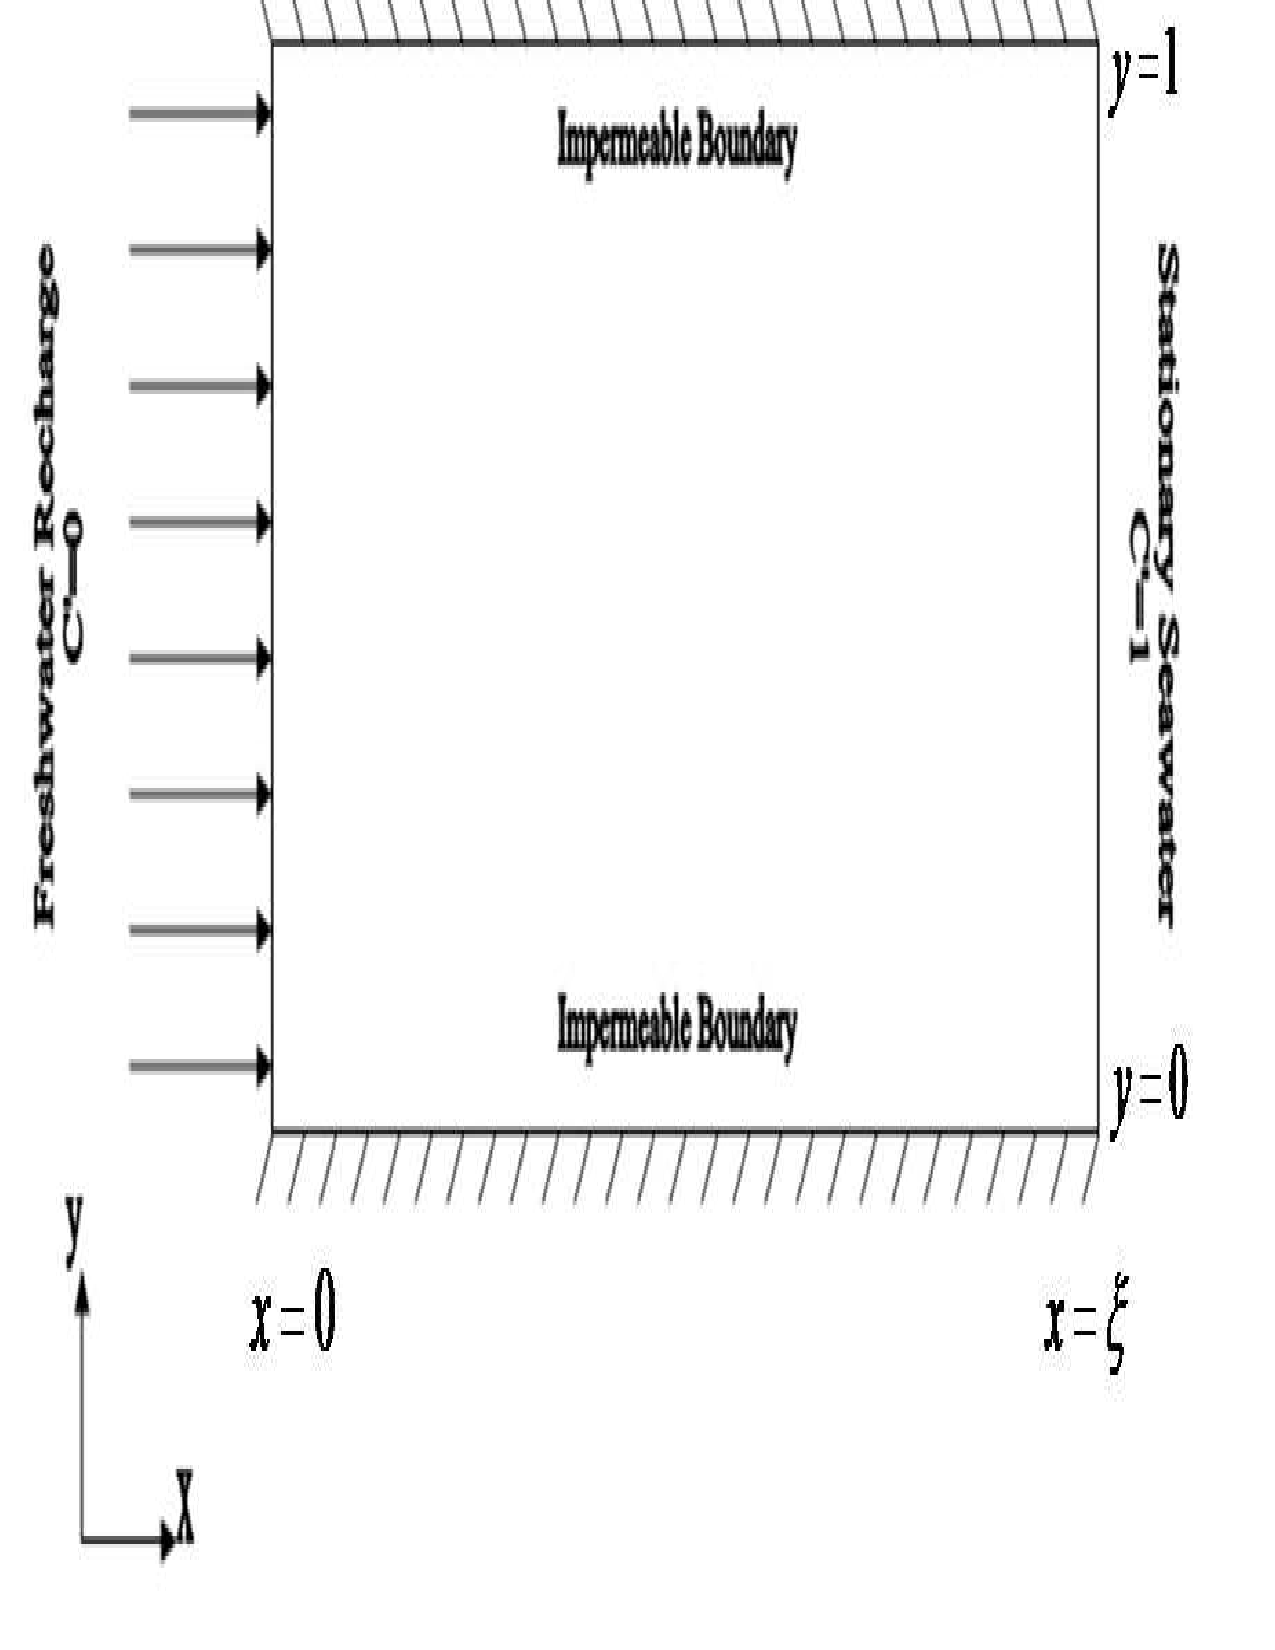
\includegraphics[totalheight=0.45 \textheight,viewport=3mm 4mm 205mm 292mm]
    {image1}
    \caption{Depiction of 2D problem domain} \label{fig:Domain}
\end{figure}

